%!TEX root = main.tex

\section{Secant Methods}
Both Newton-Raphson and Steepest descent are sound methods to compute local extrema of real-valued functions $f \colon \field{R}^d \to \field{R}$, with their pros and their cons.  
\begin{itemize}
	\item The method of Steepest descent always converges to a local minimum, yet slowly.  In order to obtain new approximations, we have to solve many different one-dimensional optimizations, each of them offering their own computational issues. 
	\item Newton offers faster sequences, but we cannot always guarantee convergence.  Another drawback of this method is the fact that we do need expressions for function itself, its gradient and Hessian matrix.  
\end{itemize}
In this section we are going to see a different concept based on the so-called \emph{secant method}, which will allow us to craft algorithms without those shortcomings.

\subsection{A secant method to search for roots of univariate functions}
To explain how it works, let's once again try to find an accurate value of $\sqrt{2}$ as the root of the polynomial $p(x) = x^2-2$.
\begin{enumerate}
	\item Consider two initial guesses $x_0=3$, $x_1=2.8$.  Notice $f(3)= 7 \neq 5.84 = f(2.8)$.
	\item The line that joins the points $(3, 7)$ and $( 2,8, 5.84)$ has equation
	\begin{align*}
	y - 7 &= \frac{5.84-7}{2.8-3}(x-3), \\ 
	y &= 5.8x-10.4.
	\end{align*}
	The latter can be seen as a linear approximation to the original function---one that did not use the derivative of $f$. This linear function intersects the $x$--axis at
	\begin{equation*}
	x_2 = \frac{10.4}{5.8} \approx 1.7931034483
	\end{equation*}
	We take this value as an approximation to the root of $f(x)=0$.
	\item Repeat this process to get a sequence of approximations $x_n$.
\end{enumerate}
\begin{example}
Observe the result of applying this recursive process, and compare with the similar experiment we conducted using the Newton-Raphson method in page \pageref{table:Newton-Raphson}.
\begin{center}
\begin{tabular}{|r|r|r|} \hline
$n$ & $x_n$ & $f(x_n)$ \\ \hline \hline
$0$ & $3.000000000000000$ & $7.0000E+00$ \\ \hline
$1$ & $2.800000000000000$ & $5.8400E+00$ \\ \hline
$2$ & $1.793103448275862$ & $1.2152E+00$ \\ \hline
$3$ & $1.528528528528528$ & $3.3640E-01$ \\ \hline
$4$ & $1.427253172054743$ & $3.7052E-02$ \\ \hline
$5$ & $1.414717869757887$ & $1.4267E-03$ \\ \hline
$6$ & $1.414215876250105$ & $6.5446E-06$ \\ \hline
$7$ & $1.414213562785585$ & $1.1667E-09$ \\ \hline
$8$ & $1.414213562373095$ & $8.8818E-16$ \\ \hline
\end{tabular}
\end{center}
\begin{figure}[ht!]
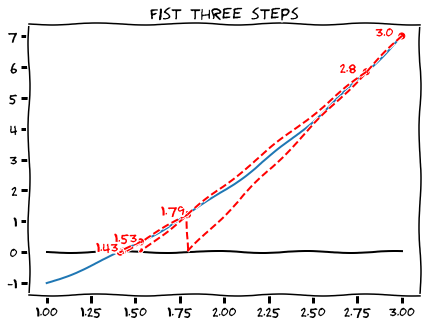
\includegraphics[width=0.6\linewidth]{images/secant.png}
\caption{Secant iterative method}\label{figure:SecantMethod}
\end{figure}
\end{example}

\begin{definition}\label{def:SecantMethod}\index{Secant method}\index{Secant method!iteration}\index{Secant method!recursive formula}
Given a function $f \colon \field{R} \to \field{R}$ and two initial guesses $x_0 \neq x_1$ satisfying $f(x_0) \neq f(x_1)$, we define the \emph{Secant method iteration} to be the sequence $\{ x_n \}_{n \in \field{N}}$ obtained by one of the following recursive formulas:
\begin{equation}\label{equation:SecantMethod}\index{Secant method!iteration}
\begin{split}
\bigg[\frac{f(x_n) - f(x_{n-1})}{x_n - x_{n-1}}\bigg] (x_{n+1} - x_{n-1}) = - f(x_{n-1}) \\
x_{n+1} = x_{n-1} - \bigg[ \frac{x_n - x_{n-1}}{f(x_n) - f(x_{n-1})} \bigg] f(x_{n-1})
\end{split}
\end{equation}
The \emph{Secant method} refers to employing this sequence to search and approximate roots of the equation $f(x)=0$.
\end{definition}